%Przykładowy plik ułatwiający złożenie projektu dyplomowego inżynierskiego.
%UWAGA: Generowany napis na stronie tytułowej o treści PROJEKT DYPLOMOWY INŻYNIERSKI został zaproponowany przeze mnie i nie jest, póki co, potwierdzony przez władze wydziału. Przed ostatecznym oddaniem tak złożonej pracy należy upewnić się jaka powinna być treść tego napisu. W momencie gdy uzyskam informację na temat treści tego napisu, dokonam niezbędnych zmian w źródłach.

\documentclass[eng,printmode]{mgr}
%opcje klasy dokumentu mgr.cls zostały opisane w dołączonej instrukcji

%poniżej deklaracje użycia pakietów, usunąć to co jest niepotrzebne
%\usepackage{polski} %przydatne podczas składania dokumentów w j. polskim
\usepackage{polski}
\usepackage[utf8]{inputenc}
\usepackage[T1]{fontenc} %poprawne składanie polskich czcionek
%pakiety do grafiki
\usepackage{graphicx}
\usepackage{subfigure}
\usepackage{psfrag}

%pakiety dodające dużo dodatkowych poleceń matematycznych
\usepackage{amsmath}
\usepackage{amsfonts}

%pakiety wspomagające i poprawiające składanie tabel
\usepackage{supertabular}
\usepackage{array}
\usepackage{tabularx}
\usepackage{hhline}

%pakiet wypisujący na marginesie etykiety równań i rysunków zdefiniowanych przez \label{}, chcąc wygenerować finalną wersję dokumentu wystarczy usunąć poniższą linię
\usepackage{showlabels}

%definicje własnych poleceń
\newcommand{\R}{I\!\!R} %symbol liczb rzeczywistych, działa tylko w trybie matematycznym
\newtheorem{theorem}{Twierdzenie}[section] %nowe otoczenie do składania twierdzeń

%dane do złożenia strony tytułowej
\title{System lokalizacji samolot\.'ow z wykorzystaniem ADS-B}
\engtitle{Airplane tracking system using ADS-B}
\author{Karol Szpila}
\supervisor{\vfil dr in\.z. Krzysztof Halawa\\
\\ Katedra Informatyki Technicznej}
%\guardian{dr hab. inż. Imię Nazwisko Prof. PWr, I-6} %nie używać jeśli opiekun jest tą samą osobą co prowadzący pracę

%\date{2008} %standardowo u dołu strony tytułowej umieszczany jest bieżący rok, to polecenie pozwala wstawić dowolny rok

%poniżej jest lista kierunków i specjalności na wydziale elektroniki, należy wybrać właściwe lub dopisać jeśli nie ma odpowiednich
\field{Automatyka i Robotyka (AIR)}
\specialisation{Technologie Informacyjne\\ w Systemach Automatyki (ART)}
%\specialisation{Robotyka (ARR)}
%\specialisation{Komputerowe sieci sterowania (ARK)}
%\specialisation{Systemy informatyczne w automatyce (ASI)}
%\specialisation{Komputerowe systemy zarządzania \\procesami produkcyjnymi (ARS)}
%\field{Elektronika i telekomunikacja (EIT)}
%\specialisation{Akustyka (ETA)}
%\specialisation{Aparatura elektroniczna (EAE)}
%\specialisation{Elektroniczne i komputerowe \\systemy automatyki (ESA)}
%\specialisation{Zastosowania inżynierii komputerowej \\w technice (EZI)}
%\specialisation{Inżynieria dźwięku (EID)}
%\specialisation{Elektronika stosowana \\i optokomunikacja (TEO)}
%\specialisation{Telekomunikacyjne sieci szerokopasmowe (TSS)}
%\specialisation{Teleinformatyczne sieci mobilne (TSM)}
%\specialisation{Sygnały w telekomunikacji cyfrowej (TSC)}
%\specialisation{Teleinformatyczne systemy rozsiewcze (TSR)}
%\field{Informatyka (INF)}
%\specialisation{Systemy informatyki w medycynie \\i technice (IMT)}
%\specialisation{Inżynieria systemów informatycznych (INS)}
%\specialisation{Inżynieria internetowa (INT)}
%\specialisation{Systemy i sieci komputerowe (ISK)}
%\field{Teleinformatyka (TIN)}
%\specialisation{Teleinformatyka (TIN)}

%tutaj zaczyna się właściwa treść dokumentu
\begin{document}
%\bibliographystyle{plabbrv} %tylko gdy używamy BibTeXa, ustawia polski styl bibliografii

\maketitle %polecenie generujące stronę tytułową
%\dedication{6cm}{To jest przykładowa treść opcjonalnej dedykacji, należy ją zmienić lub usunąć w całości polecenie \texttt{$\backslash$dedication}}

\tableofcontents %spis treści

%poniżej znajduje się przykładowa treść dalszej części dokumentu, zainteresowanych zachęcam do rozszyfrowania frazy "Lorem ipsum" :)
\let\cleardoublepage\clearpage %usuwa puste strony pomiaedzy rozdziałami

\chapter{ Wstęp }

\subsection{Automatic dependent surveillance – broadcast}
ADS-B jest systemem śledzenia położenia statków powietrznych mający uzupełiac pracę PSR (eng. Primary Surveilance Radar). PSR to radar aktywny bazujący na wysyłaniu fal elektromagnetycznych oraz pomiarze czasu powrotu fali odbitej od obiektu. Wadą takich systemów jest brak informacji o wykrytym obiekcie poza jego lokalizacją i rozmiarem. ADS-B polega na automatycznym wysyłaniu pozycji statku powietrznego określonego przy pomocy pokładowego systemu GPS w przestrzeń, tak że zarówno kontrola naziemna jak i pobliskie samoloty są w stanie odebrać tą wiadomość. 

\chapter{ Cele i założenia projektowe }
Celem niniejszej pracy by\l{}o zbudowanie prototypu systemu pozwalającego na lokalizację oraz zbieranie informacji o  statkach powietrznych wyposażonych w nadajniki ADS-B.                                                                                                                                                                                                                                                                                                                                                            
\chapter{ Realizacja projektu }
\section{ Warstwa sprzętowa}
W tym rozdziale zostanie opisana czę\'s\'c sprzętowa projektu, czyli schemat urządzenia oraz projekt PCB, wykorzystane elementy oraz zewnętrzne urządzenia.
\subsection{Zasilanie}
Urządzenie jest zasilanie z zewnętrznego źródła 5V poprzez port USB typu mini A. Pozwala to na podłącznie PCB zarówno do sieci przy pomocy ładowarki do telefonu jak i z komputera czy z przenośnego power banku. Ponieważ układy takie jak mikrokontroler czy pamieć SDRAM potrzebują napięcia 3.3V zastosowano stabilizator LM1117 Poniżej przedstawiono schemat podłączania.

\begin{figure}[!h]
    \centering
    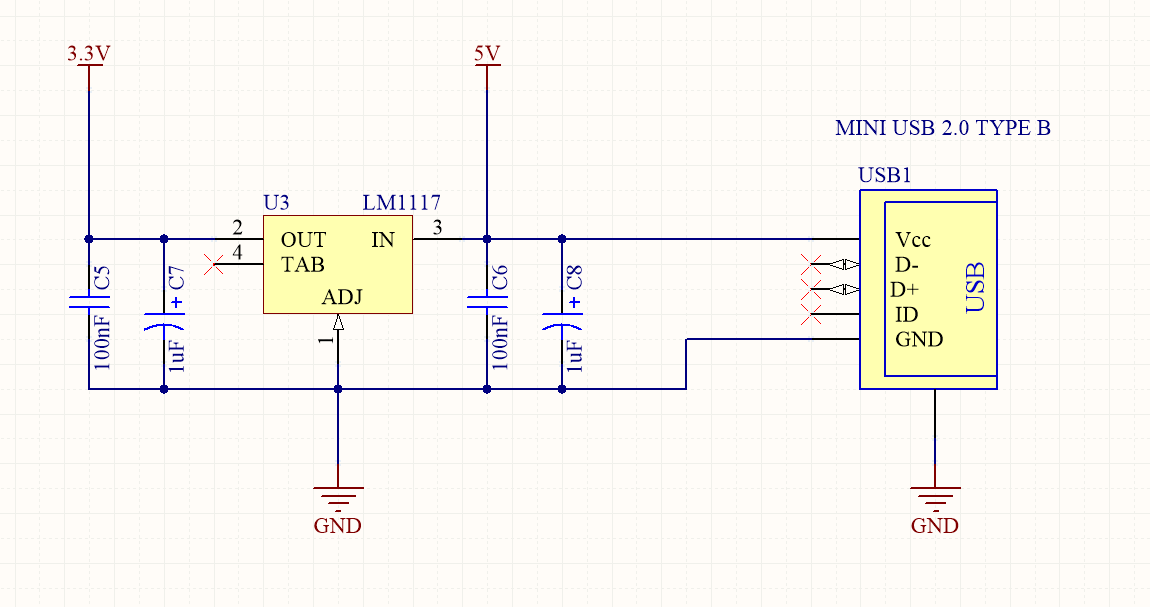
\includegraphics[width=\textwidth]{schematics/power.png}
    \caption{\textit{\scriptsize Schemat zasilania płZytki PCB}}
\end{figure}
\subsection{Mikrokontroler}
Wykorzystany mikrokontroler to STM32F767ZIT6. Układ został wybrany ze względu na zmieszczenie w najmniejszej obudowie wszystkich wymaganych układów peryferiów takich jak: kontroler LDTC do sprzętowej obsługi wyświetlacza LCD, kontroler pozwalający obsłużyć zewnętrzną pamięcią SDRAM i interfejsy komunikacyjne USB, I2C i UART. Poniżej przedstawiono schemat podłączenia.

\begin{figure}[!h]
    \centering
    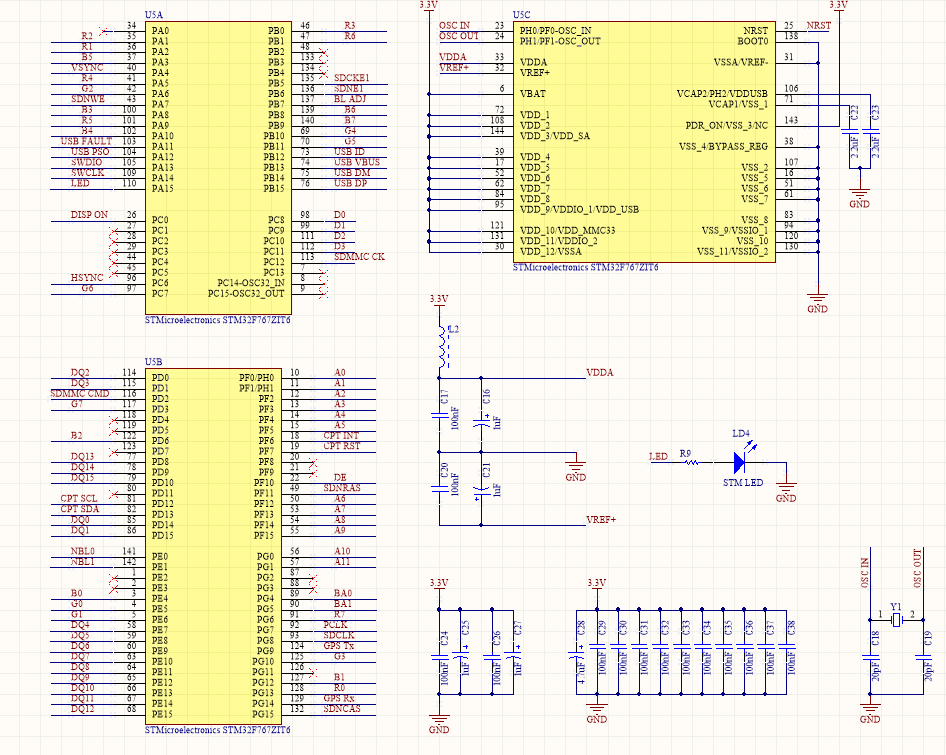
\includegraphics[height=\textwidth, angle=90]{schematics/uC.png}
    \caption{\textit{\scriptsize Schemat podłączenia mikrokontrolera STM32f767ZIT6}}
\end{figure}

\subsection{Pamięć SDRAM}
Do systemu dodano zewnętrzą pamięć SDRAM do buforowania ramek przekazywanych do wyświtlacza. Wewnętrza pamieć SRAM mikrokontrolera była niewystarczająca. Zdecydowano się na układ IS42S16400J-7TLI. Poniżej przedstawiono schemat podłaczenia.

\begin{figure}[!h]
    \centering
    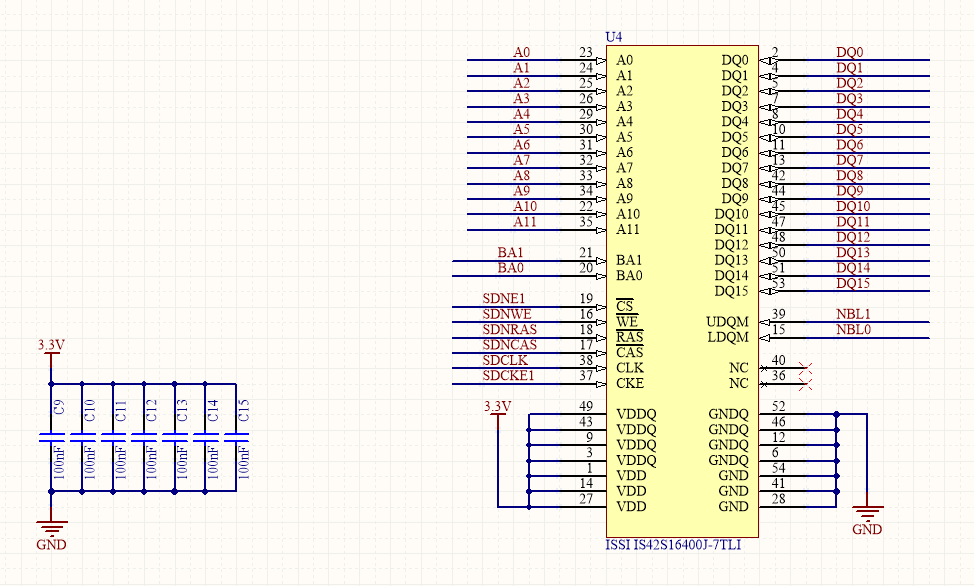
\includegraphics[width=\textwidth]{schematics/sdram.png}
    \caption{\textit{\scriptsize Schemat podłączenia zewnętrzej pamięci SDRAM}}
\end{figure}

\subsection{Moduł GPS}
Aby system był w stanie popranie obliczyć odległość od namierzonego statu powietrznego i poprawnie zaznaczyć jego pozycję na radarze, potrzebna znać pozycje urządzenia. Do tego zadania wybrano układ NEO-6M-0-001 z zewnętrzną aktywną anteną. Układ posiada baterie podtrzymującą napięcie zasilania.

\begin{figure}[!h]
    \centering
    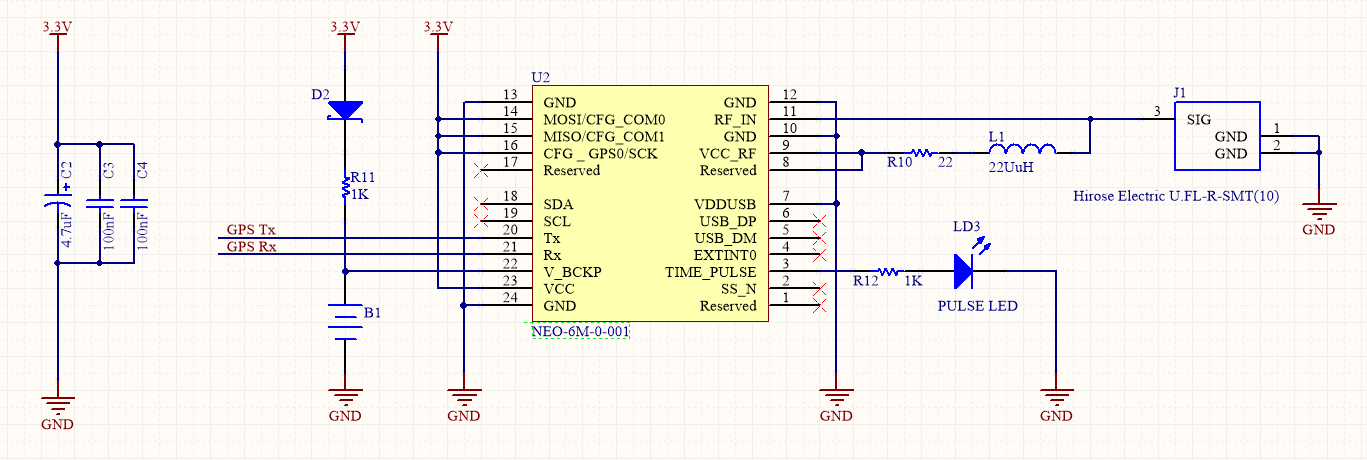
\includegraphics[width=\textwidth]{schematics/gps.png}
    \caption{\textit{\scriptsize Schemat podłączenia modułu GPS}}
\end{figure}

\subsection{Wyswietlacz}
Formę interfejsu graficznego dla użytkownika pełni 10,1" wyświetlacz HYC o rozdzielczości 1024 na 600 piskeli
%dopisac cos o rbg i dopasowanii
\begin{figure}[!h]
    \centering
    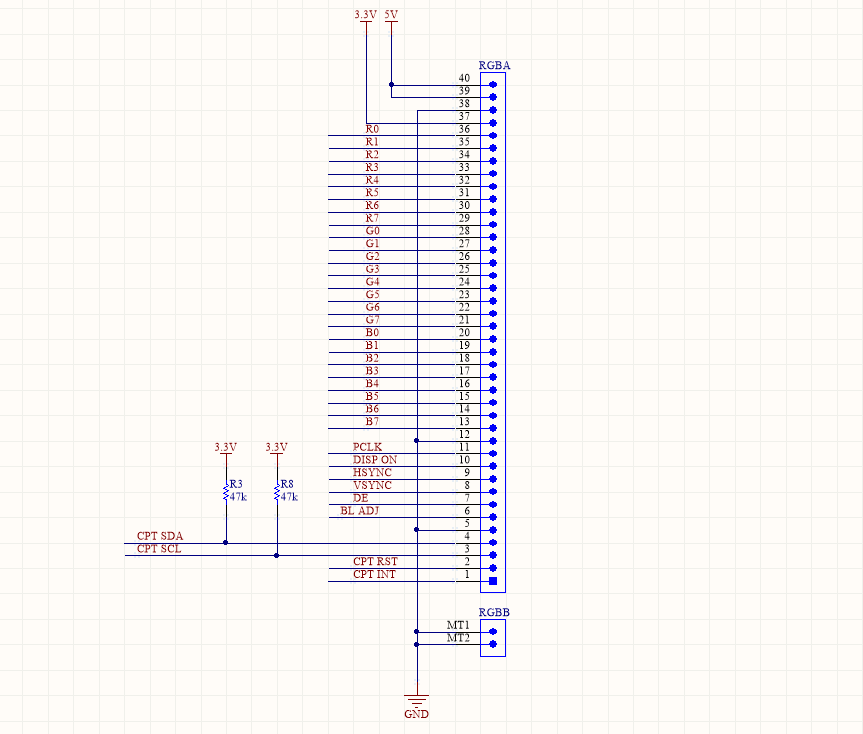
\includegraphics[width=\textwidth]{schematics/display.png}
    \caption{\textit{\scriptsize Schemat podłączenia wyswietlacza}}
\end{figure}

\subsection{Interfejsy komunikacyjne}
System posiada gniazdo na kartę Micro SD, która może zostać wykorzysta do przechowywania skompresowanych obrazów do tła GUI lub co planowane jest w przyszłości map pozwalających lepiej orientować się w terenie na podstawie obrazu z radaru. Do programowania mikrokontrolera wykorzystany został dedykowany dwuprzeowodowy interfejs SWD zgodny z ST-Link. Ostatni zostanie omówiony interfejs USB do komunikacji z SDR (eng Software Defined Radio). Interfejs został wyprowadzony poprzez gniazdo Micro USB-B pozwalając w ten sposób zaoszczędzić miejsca na PCB. System jako Host USB będzie zasilać podłączony układy których pobór nie powinien przekroczyć, zgodznie ze stangardem USB2.0 500mA ,dlatego zastosowano power switch STMPS2141STR. W przypadku podania stanu wysokiego na pin USB PSO switch zostanie właczony. Jeżeli nie występują żadne sytuacje nieporządne takie jak przetężenie prądowe czy zwarcie, zapali się zielona dioda sygnalizująca poprawnie działanie zasilania. W przypadku jakichkolwiek problemów prąd zostanie natychmiast odcięty a układ wystawi wysoki stan na pin FAULT informując mikrokontroler i zapalając czerwona diodę. W celu zabezpieczania interfejsu przed nieporządanymi wyładowaniami elektrostatycznymi związanymi z dotykaniem urządzenia czy wkładaniem urządzenia do gniazda zastosowano układ ochrony ESD (ang . Electro Static Discharge ) STMECMF02-4CMX8 dedykowany dla USB2.0.
 %sprawdzic czy prawda z h na faul

\begin{figure}[!h]
    \centering
    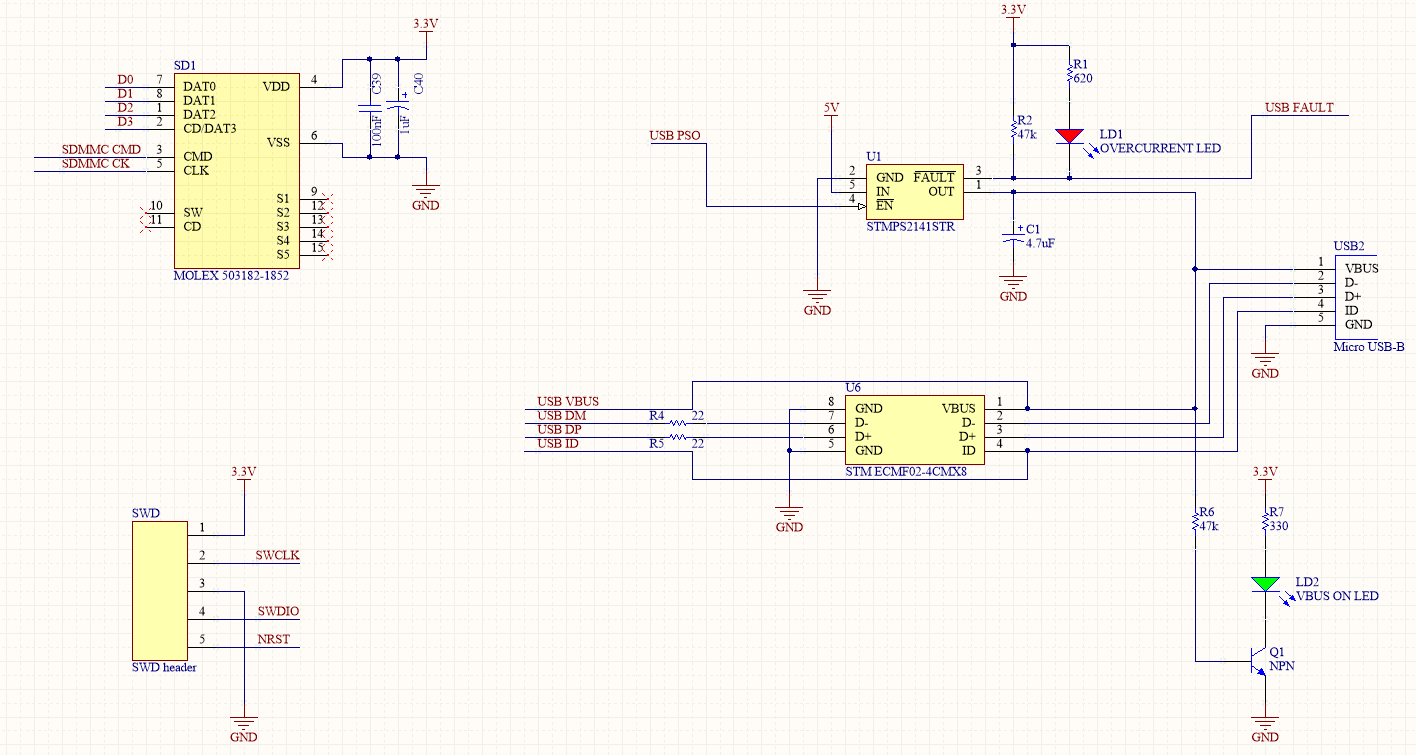
\includegraphics[width=\textwidth]{schematics/conn.png}
    \caption{\textit{\scriptsize Schemat podłączenia zewnętrych interfejsów}}
\end{figure}
\section{ Warstwa Programowa }
\subsection{System Operacyjny}

\chapter{ Podsumowanie }


\addcontentsline{toc}{chapter}{Bibliografia} %utworzenie w spisie treści pozycji Bibliografia
\bibliography{bibliografia} % wstawia bibliografię korzystając z pliku bibliografia.bib - dotyczy BibTeXa, jeżeli nie korzystamy z BibTeXa należy użyć otoczenia thebibliography

%opcjonalnie może się tu pojawić spis rysunków i tabel
% \listoffigures
% \listoftables
\end{document}
